\documentclass[10pt, a4paper]{article}
\usepackage[margin=2.2cm]{geometry}
\usepackage{amsmath, amssymb}
\usepackage{booktabs}
\usepackage{graphicx}
\graphicspath{{figures/}}
\usepackage[hidelinks]{hyperref}
\usepackage{caption}
\usepackage{tikz}
\usetikzlibrary{positioning, arrows.meta, calc}
\usepackage{microtype}
\usepackage{fancyhdr}
\usepackage{titlesec}
\usepackage{abstract}
\usepackage{xcolor}
\usepackage{array}
\usepackage{enumitem}
\usepackage{colortbl}
\usepackage{multirow}
\usepackage[numbers]{natbib}
\definecolor{darkgray}{RGB}{40,40,40}
\definecolor{medgray}{RGB}{120,120,120}
\definecolor{lightgray}{RGB}{245,245,245}
\definecolor{accentblack}{RGB}{15,15,15}
\titleformat{\section}{\normalsize\bfseries\scshape\color{accentblack}}{\thesection.}{0.5em}{}[{\color{medgray}\titlerule[0.4pt]}]
\titleformat{\subsection}{\normalsize\bfseries\color{darkgray}}{\thesubsection}{0.5em}{}
\titlespacing{\section}{0pt}{10pt}{5pt}
\titlespacing{\subsection}{0pt}{6pt}{3pt}
\renewcommand{\abstractnamefont}{\normalfont\bfseries\scshape\small}
\renewcommand{\abstracttextfont}{\normalfont\small}
\captionsetup{font=small, labelfont=bf, labelsep=period, skip=6pt}
\pagestyle{fancy}
\fancyhf{}
\renewcommand{\headrulewidth}{0.4pt}
\lhead{\small\scshape\color{medgray} GNet: Visual and Audio-Visual Lip Reading for German}
\rhead{\small\color{medgray}\thepage}
\setlength{\parskip}{4pt}
\setlength{\parindent}{1em}
\setlength{\absleftindent}{0pt}
\setlength{\absrightindent}{0pt}
\renewcommand{\topfraction}{0.9}
\renewcommand{\bottomfraction}{0.8}
\renewcommand{\textfraction}{0.07}
\renewcommand{\floatpagefraction}{0.7}
\setcounter{topnumber}{4}
\setcounter{bottomnumber}{2}
\setcounter{totalnumber}{6}
\begin{document}
\vspace*{0.5em}
{\centering
    {\Large\bfseries\scshape GNet: Visual and Audio-Visual Lip Reading for German Word Classification}\\[0.5em]
    {\large Peter Staykov}\\[1.0em]
}
\noindent\rule{\textwidth}{1pt}
\begin{abstract}
\noindent
GNet is a visual lip-reading model for German word-level classification, trained on GLips, a corpus of about 250{,}000 clips of Hessian Parliament speakers covering 500 word classes. It couples a 3D-CNN and ResNet-18 visual frontend with a lightweight temporal back-end: a multi-scale depthwise convolutional stem followed by a two-layer Transformer encoder, compared against an MS-TCN back-end sharing the same frontend, data pipeline and training recipe. On the 15-word GLips benchmark GNet reaches $59.3\%$ top-1 accuracy from scratch, ahead of previously published results on the same corpus and split. In-domain GLips-498 to GLips-15 transfer lifts this to $69.5\%$, a new baseline for in-domain transfer on this benchmark rather than a direct comparison to prior cross-lingual transfer, which uses a different setting and an unpublished word draw. On the full vocabulary GNet reaches $34.2\%$ top-1 accuracy (500 classes, after fixing a preprocessing bug affecting 2 classes; see Section~\ref{sec:results}). Controlled ablations trace this improvement mainly to preprocessing and training data rather than architecture: mouth-ROI cropping is by far the largest single factor, the two back-ends perform comparably at 15 words, and the Transformer's advantage is limited to the full vocabulary at a meaningfully smaller parameter count. Negative results are reported in full, including an attentive-pooling head that does not outperform mean pooling.
\noindent GNet's frozen visual encoder is further paired with a frozen Whisper speech encoder \citep{radford2022whisper}, raising full-vocabulary accuracy from $33.5\%$ visual-only to $73.0\%$ top-1 on the held-out test split, the first published audio-visual figure for GLips at any vocabulary size. Four fusion mechanisms are compared under an identical frozen-backbone, cached-token protocol, isolating the fusion architecture from the frontends: late score-summation, feature concatenation, gated cross-attention (also evaluated as a separately fine-tuned end-to-end architecture), and an AV-HuBERT-style \citep{shi2022avhubert} joint Transformer over concatenated modality tokens with full cross-modal self-attention. The two attention-based mechanisms clear both naive ones by a wide margin; the naive mechanisms just track an audio-only probe on the same frozen features at clean audio and only draw on vision once noise is introduced. Under additive white and babble noise the joint Transformer degrades gradually and stays ahead of naive fusion throughout, while the audio-only probe eventually falls below the visual-only floor at the harshest condition tested. Freezing both backbones and training only a small fusion head matches a fully fine-tuned end-to-end replica of the cross-attention architecture on fused accuracy, while keeping the exact visual-only fallback that the fine-tuned model's own fallback lacks.
\end{abstract}
\noindent\rule{\textwidth}{0.4pt}
\vspace{0.8em}
\section{Introduction}
\noindent Visual speech recognition (VSR), the classification of spoken words from silent video of a speaker's face, has advanced rapidly on English benchmarks such as LRW, but progress in other languages remains limited by data availability. For German the only word-level benchmark is GLips \citep{schwiebert2022glips}, and published results on it cover a 15-word subset only: $50.9\%$ top-1 accuracy training from scratch, and $54.8\%$ when transferring from the larger English LRW corpus. No result has been reported for the full 500-word vocabulary, no study has isolated the contribution of the temporal back-end under a fixed frontend and training recipe, and no published system fuses vision with audio on this corpus at all, despite GLips clips carrying a usable audio track.
\noindent All three gaps are addressed here. GNet is a lip-reading model whose visual frontend follows the standard design for word-level VSR (a single spatiotemporal convolution followed by a per-frame ResNet-18) and whose temporal back-end is a multi-scale depthwise convolutional stem feeding a shallow Transformer encoder. With the frontend, the data pipeline, the augmentation stack and the optimiser settings held fixed, only the temporal module is substituted for an MS-TCN baseline, so that reported accuracy differences are attributable to the back-end design rather than to incidental changes elsewhere in the recipe. The same matched pair is evaluated across three settings: the full vocabulary, the 15-word subset from scratch, and GLips-498 to GLips-15 in-domain transfer, with architecture and preprocessing ablations in addition. GNet's frozen visual encoder is then paired with a frozen Whisper speech encoder \citep{radford2022whisper} under four fusion mechanisms, compared under an identical cached-token protocol so that the comparison isolates the fusion architecture rather than the frontends, with noise-robustness and frozen-versus-fine-tuned comparisons in addition.
\noindent Adding a frozen Whisper encoder and a small joint-attention fusion head raises full-vocabulary top-1 accuracy from $33.5\%$ to $73.0\%$, a gain an order of magnitude larger than any visual-only architectural difference measured here. GNet on its own also exceeds the published visual results on this benchmark by a substantial margin, using a larger parameter count and tracked mouth-ROI cropping than the lighter, detection-free pipeline it is compared against. The ablations below trace the improvement mainly to this preprocessing and to training data rather than architecture: on the 15-word task the two back-ends differ by only $0.1$ points, while removing the mouth-ROI crop costs $29.2$. The Transformer's advantage is confined to the full-vocabulary task ($+5.3$ points, at a $2.9\times$ smaller temporal module), so it reads as a parameter-efficiency result with a large-vocabulary accuracy benefit rather than a general one. The core contributions:
\begin{itemize}[leftmargin=1.4em, itemsep=2pt]
    \item \textbf{The first audio-visual result on GLips, at any vocabulary size.} A small joint-attention head over frozen visual and audio encoders reaches $73.0\%$ top-1 on the held-out test split (Table~\ref{tab:mm}).
    \item \textbf{A controlled comparison of four fusion mechanisms}, under identical frozen backbones, cached tokens and recipe: late score-summation, feature concatenation, gated cross-attention, and an AV-HuBERT-style \citep{shi2022avhubert} joint Transformer. The two attention-based heads clear both naive ones by a wide margin; the naive heads just track the audio-only probe at clean audio.
    \item \textbf{Noise robustness and a frozen-versus-fine-tuned comparison.} Attention-based fusion stays ahead of naive fusion at every tested noise level, and a frozen backbone with a light fusion head matches full end-to-end fine-tuning on fused accuracy without losing the visual-only fallback that fine-tuning otherwise degrades.
    \item \textbf{New best published results on GLips-15.} GNet reaches $59.3\%$ top-1 from scratch, ahead of both prior published pipelines on the same split. In-domain transfer and a two-back-end ensemble push this further.
    \item \textbf{First full-vocabulary visual-only GLips benchmark}, with a matched MS-TCN baseline, serving as the floor the audio-visual fusion above is measured against.
    \item \textbf{In-domain transfer as an alternative to cross-lingual transfer.} Pretraining on the full vocabulary and fine-tuning on the 15-word subset beats training from scratch by a wide margin. This is not directly comparable to the published cross-lingual result, so it is treated as a new in-domain baseline rather than a like-for-like win.
    \item \textbf{A controlled MS-TCN and Transformer ablation.} Both back-ends share the frontend, data, augmentation and optimiser. The Transformer's advantage is confined to the full vocabulary, where it is also the more parameter-efficient design.
    \item \textbf{An accounting of the improvement's sources, including negative results.} Ablations isolate mouth-ROI preprocessing as the dominant factor, with a smaller contribution from the convolutional stem and no gain from attentive pooling over mean pooling.
\end{itemize}
\section{Related Work}
\subsection{Architectures for large-vocabulary visual speech recognition}
\noindent GNet's frontend and one of its two temporal back-ends derive from the LRW and LRW-1000 literature. \citet{stafylakis2017combining} established the standard frontend: a single spatiotemporal convolution over short frame windows, followed by a per-frame 2D ResNet and a recurrent temporal model. \citet{martinez2020lipreading} replaced the recurrent back-end with a multi-scale temporal convolutional network (MS-TCN), simplifying training to a single stage, improving generalisation across sequence lengths, and setting state-of-the-art results on LRW and LRW-1000. This 3D-CNN, ResNet-18 and MS-TCN combination is the direct ancestor of both of GNet's configurations. Later work extended the convolutional line: the densely connected TCN of \citet{ma2021densely} added skip connections between blocks to widen the temporal receptive field, and more recent multi-dilated variants match or exceed TCN accuracy at lower parameter cost \citep{lee2025td3net}. Attention- and Transformer-based back-ends form a separate line, replacing the recurrent or convolutional temporal module outright \citep{prajwal2022subword}.
\noindent GNet combines both approaches, a multi-scale convolutional stem with a shallow Transformer encoder on top, and reports both back-ends as a matched pair rather than a single substitution. None of the cited work runs a controlled MS-TCN and Transformer comparison holding data, frontend and training recipe fixed; architectural changes there are evaluated against a fixed prior baseline, which confounds the back-end's contribution with concurrent changes in the training procedure. That confound looks material here: under a matched recipe the back-end gap is small and does not consistently favour one family.
\subsection{German visual speech recognition}
\noindent \citet{schwiebert2022glips} introduced GLips, approximately $250{,}000$ clips of Hessian Parliament speakers over $500$ word classes, formatted to match LRW so that cross-lingual transfer is possible, and showed that LRW to GLips transfer improves both convergence speed and final accuracy relative to training from scratch. Their pipeline also crops to a lip region of interest per frame prior to recognition, a preprocessing choice the ablations in Section~\ref{sec:results} confirm is highly consequential. Their work established the first German VSR baseline, but on a 15-class subset only, via cross-lingual transfer only, and without a full-vocabulary result. The reported figures are $50.9\%$ top-1 accuracy from scratch and $54.8\%$ with LRW pretraining.
\noindent \citet{ameer2024} benchmark a NASNetMobile-based pipeline on the same 15-class GLips subset, running a 16-configuration sweep crossing four pretrained 2D backbones with four temporal back-ends, and comparing against two further structured-dataset baselines. Their best configuration (NASNetMobile with a CNN back-end, $4.68$M parameters) reaches $48.4\%$ accuracy and $0.485$ macro-$F_1$ without in-domain transfer.
\noindent The two pipelines differ substantially in preprocessing. \citet{ameer2024} avoid face detection, processing uncropped frames at $128\times128$ with image- and feature-level augmentation, on the grounds that cropping discards information relevant to unconstrained data. GNet uses MediaPipe FaceMesh \citep{lugaresi2019mediapipe} to extract a tracked, scale-normalised mouth crop per frame (Section~\ref{sec:pre}). The effect of this choice is quantified in Section~\ref{sec:results}, where it emerges as the largest single factor in the results, and a capacity stress-test of this architecture under uncropped input is reported in Section~\ref{sec:ameer}.
\subsection{Audio-visual fusion for speech recognition}
\label{sec:relwork-av}
\noindent Combining vision with audio is well established for English speech recognition under noise. \citet{afouras2018deep} show that a jointly trained audio-visual Transformer improves over audio-only ASR specifically as acoustic noise increases, since the two modalities are corrupted by largely independent noise sources. \citet{shi2022avhubert} take this further with AV-HuBERT, which concatenates visual and audio token sequences with modality-type embeddings and processes them with a single shared Transformer under masked cluster-prediction pretraining, learning cross-modal structure through full self-attention rather than a hand-designed cross-attention module. The \texttt{joint\_tf} fusion head in Section~\ref{sec:mm} follows this concatenate-and-self-attend design at inference time, though without AV-HuBERT's masked pretraining stage. \citet{afouras2018deep} instead fuse the modalities through explicit encoder-decoder attention, one modality's representation attending over the other's rather than joint self-attention over a concatenated sequence; the gated cross-attention head compared here follows that design in simplified, single-layer form. \citet{radford2022whisper} is used here as a fixed, off-the-shelf audio feature extractor (Whisper, trained on large-scale weakly-supervised multilingual audio) rather than as a component trained jointly with the visual model, so that the audio pathway itself is held constant across every fusion mechanism compared and the comparison isolates the fusion architecture.
\subsection{Summary of the gap addressed}
\noindent No prior study on GLips, including the dataset paper, the sweep of \citet{ameer2024}, or the structured-dataset baselines they cite, evaluates the full vocabulary, runs a matched MS-TCN and Transformer ablation, compares in-domain transfer (GLips-498 to GLips-15) against the cross-lingual LRW transfer that has so far been the only transfer result reported for this corpus, or fuses audio with vision at all. GNet is narrower than \citet{ameer2024} in backbone diversity and relies on landmark-tracked mouth-ROI cropping, as in \citet{schwiebert2022glips}, rather than their detection-free design. To the best of available knowledge it is nonetheless the first work to vary vocabulary size, transfer setting and back-end architecture together in a controlled comparison on GLips, and the first to report an audio-visual result on this corpus at all.
\section{Method}
\label{sec:arch}
\noindent The visual encoder is defined once and reused unchanged for both temporal back-ends, so that the comparison controls for the visual pathway and targets the temporal model as the variable of interest. Note that the ResNet backbone is fine-tuned rather than frozen during training (Section~\ref{sec:train}), so the two configurations share an architecture and recipe rather than a single set of trained weights; back-end-dependent gradient dynamics could in principle shape the learned visual features differently for each back-end, and the comparison below should be read on those terms rather than as a strict causal isolation of the temporal module alone.
\paragraph{Shared visual encoder.}
An input clip $x \in \mathbb{R}^{3 \times T \times H \times W}$ is processed by a \emph{Frontend3D}, a single 3D convolution with kernel $k=(5,7,7)$ and stride $(1,2,2)$ that preserves the temporal axis while halving the spatial axes, followed by batch normalisation, ReLU and a spatial max-pool. Each of the $T$ frames is then passed independently through the ImageNet-pretrained ResNet-18 stages (\texttt{layer1} to \texttt{layer4}), yielding a per-frame feature $f_t \in \mathbb{R}^{512}$ after global spatial average pooling. GLips clips are $1.16\,\mathrm{s}$ at $25\,\mathrm{fps}$; $T = 25$ frames per clip are sampled at $H = W = 88$. Both back-ends consume the same feature sequence $F \in \mathbb{R}^{T \times 512}$, and the encoder accounts for $11.2$M of each model's parameters.
\paragraph{Temporal back-end (GNet).}
$F$ passes through (i) a linear projection $\mathrm{Linear}(512 \to d) + \mathrm{LayerNorm}$ with $d = 256$; (ii) a multi-scale convolutional stem of two \texttt{MSTemporalBlock}s, each averaging three parallel depthwise branches with kernels $k \in \{3,5,7\}$, where each branch comprises a depthwise convolution, a pointwise convolution, batch normalisation and GELU, under a residual connection and LayerNorm; (iii) a learned positional embedding; (iv) a $2$-layer pre-norm Transformer encoder ($8$ heads, FFN width $1024$, GELU, dropout $0.2$); and (v) attentive temporal pooling followed by dropout and a linear classifier. Attentive pooling scores each token with a small two-layer network $g$, forms weights $w_t = \mathrm{softmax}\big(g(z_t)\big)$, and returns $\sum_t w_t\, z_t$. The temporal module totals $2.2$M parameters, giving $13.4$M for the whole model on the 15-class task.
\paragraph{Temporal back-end (MS-TCN baseline).}
The same $F$ is fed to a multi-scale temporal convolutional network operating directly on the $512$-d sequence. It stacks $B = 4$ MS-TCN blocks of width $384$; each block runs parallel 1-D temporal convolutions with kernels $k \in \{3,5,7\}$ at increasing dilation, followed by batch normalisation, ReLU and a residual connection. A final temporal average pool over $T$ feeds a linear classifier. With no attention but wider channels, the baseline's temporal module uses $6.4$M parameters against $2.2$M for GNet, and $17.6$M against $13.4$M overall.
\subsection{Design rationale}
\noindent Because both back-ends share the encoder design, the accuracy gap between them is attributable mainly to the temporal model, with the caveat above about end-to-end fine-tuning of the shared backbone. The frontend, a single spatiotemporal convolution followed by a per-frame ResNet, is the standard design for word-level VSR, introduced by \citet{stafylakis2017combining} and reused by subsequent LRW systems \citep{martinez2020lipreading, ma2021densely}; keeping it unchanged is what keeps the comparison focused on the back-end.
\noindent\emph{Temporal stride $1$ in the Frontend3D.} The frontend convolves over short windows (kernel $k=(5,7,7)$) at unit temporal stride, so that no frames are merged before the back-end, preserving the short-range articulatory dynamics that separate visually similar words. The same short-window, unit-stride design underlies the canonical LRW frontend \citep{stafylakis2017combining} and the sub-clip encoders used in more recent attention-based systems \citep{prajwal2022subword}.
\noindent\emph{Multi-scale depthwise branches ($k\in\{3,5,7\}$).} Multi-scale temporal convolution is the basis of the TCN back-end's competitiveness: \citet{martinez2020lipreading} improved over the recurrent baseline by mixing short and long temporal receptive fields, and dense or dilated successors \citep{ma2021densely, lee2025td3net} indicate that broad receptive-field coverage, rather than depth, is the principal accuracy lever, and that it can be obtained at low cost. The depthwise branches used here are an inexpensive realisation of this principle; their contribution is measured in Section~\ref{sec:results} at $2.4$ points of top-1 accuracy.
\noindent\emph{Shallow ($2$-layer) Transformer.} GLips provides $500$ clips per class \citep{schwiebert2022glips}, that is, $400$ training clips per word under the published split, a regime in which self-attention overfits readily. The stack is capped at $2$ layers, reduced from an initial $4$ which overfit measurably, relying on dropout.
\noindent\emph{Attentive pooling.} Each clip is largely non-articulatory, since the target word occupies only a fraction of the $25$ frames, so a uniform temporal average dilutes the informative frames, and query-based attentive pooling is intended to up-weight them \citep{prajwal2022subword}. The ablation in Section~\ref{sec:results} does not support this rationale: a mean-pooling variant performs equivalently. Attentive pooling is nonetheless retained as the default configuration, since the transfer runs reported below were trained with it.
\paragraph{Transfer procedure.}
\label{sec:transfer}
GLips is designed to be LRW-compatible, and \citet{schwiebert2022glips} show that transfer between the two corpora accelerates convergence and improves accuracy. The same mechanism is applied within GLips here. For both back-ends, transfer warm-starts every tensor of the feature extractor whose name and shape match, comprising the 3D frontend, the ResNet, the temporal module, the positional embedding and the pooling head, and reinitialises only the classifier, so that a model with a different class count warm-starts cleanly (\texttt{load\_transfer\_weights}). The source is always the corresponding full-vocabulary model of the same back-end family, so the transfer comparison remains matched.
\begin{figure*}[!htb]
\centering
\resizebox{\textwidth}{!}{%
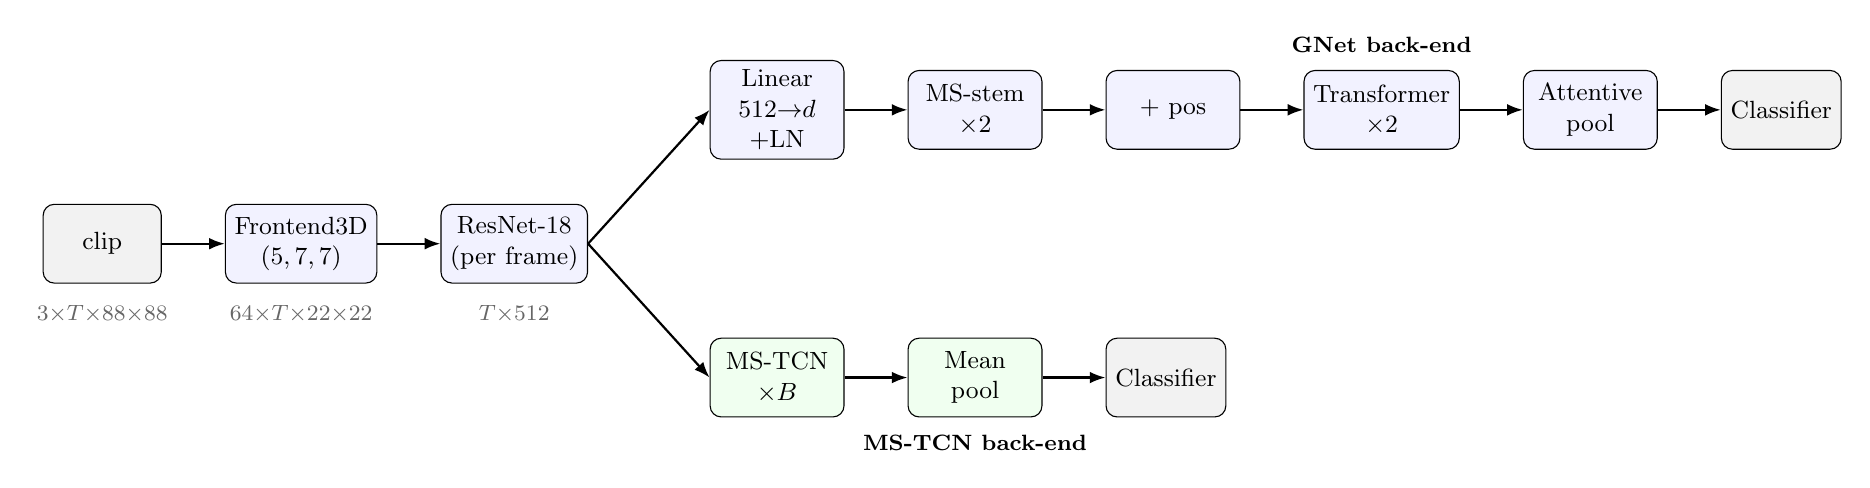
\begin{tikzpicture}[
  font=\small, node distance=8mm,
  block/.style={draw, rounded corners, minimum height=10mm, minimum width=17mm, align=center, fill=blue!5},
  tcnb/.style={draw, rounded corners, minimum height=10mm, minimum width=17mm, align=center, fill=green!6},
  io/.style={draw, rounded corners, minimum height=10mm, minimum width=15mm, align=center, fill=gray!10},
  shp/.style={font=\footnotesize\itshape, text=black!60},
  arr/.style={-{Latex[length=2mm]}, thick},
]
  % shared trunk
  \node[io]                    (clip)  {clip};
  \node[block, right=of clip]  (front) {Frontend3D\\$(5,7,7)$};
  \node[block, right=of front] (res)   {ResNet-18\\(per frame)};
  % GNet branch (top)
  \node[block] (proj) at ([shift={(2.4,1.7)}]res.east) {Linear\\$512{\to}d$\\$+$LN};
  \node[block, right=of proj] (ms)   {MS-stem\\$\times 2$};
  \node[block, right=of ms]   (pos)  {$+$ pos};
  \node[block, right=of pos]  (tr)   {Transformer\\$\times 2$};
  \node[block, right=of tr]   (pool) {Attentive\\pool};
  \node[io, right=of pool]    (cls1) {Classifier};
  % MS-TCN branch (bottom)
  \node[tcnb] (tcn) at ([shift={(2.4,-1.7)}]res.east) {MS-TCN\\$\times B$};
  \node[tcnb, right=of tcn] (mpool) {Mean\\pool};
  \node[io, right=of mpool] (cls2) {Classifier};
  % trunk arrows
  \draw[arr] (clip) -- (front);
  \draw[arr] (front) -- (res);
  \draw[arr] (res.east) -- (proj.west);
  \draw[arr] (res.east) -- (tcn.west);
  % top chain
  \foreach \a/\b in {proj/ms, ms/pos, pos/tr, tr/pool, pool/cls1} \draw[arr] (\a) -- (\b);
  % bottom chain
  \foreach \a/\b in {tcn/mpool, mpool/cls2} \draw[arr] (\a) -- (\b);
  % branch labels
  \node[font=\footnotesize\bfseries, above=1mm of tr]   {GNet back-end};
  \node[font=\footnotesize\bfseries, below=1mm of mpool] {MS-TCN back-end};
  % shape annotations
  \node[shp, below=1.5mm of clip]  {$3{\times}T{\times}88{\times}88$};
  \node[shp, below=1.5mm of front] {$64{\times}T{\times}22{\times}22$};
  \node[shp, below=1.5mm of res]   {$T{\times}512$};
\end{tikzpicture}}
\vspace{3mm}
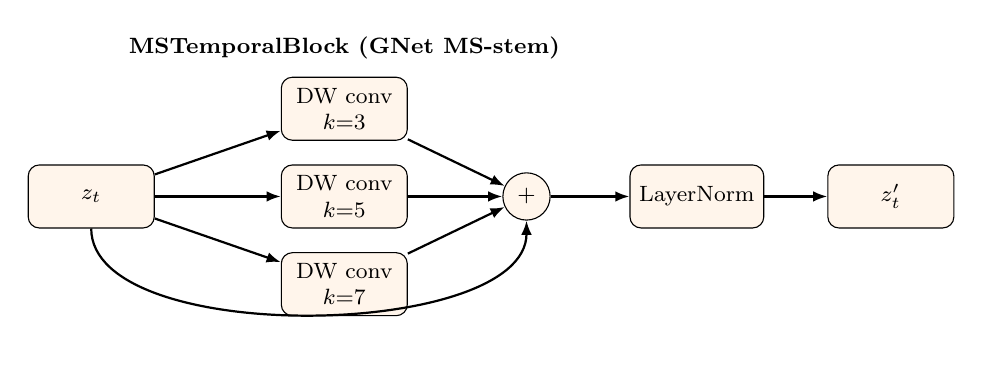
\begin{tikzpicture}[
  font=\footnotesize,
  block/.style={draw, rounded corners, minimum height=8mm, minimum width=16mm, align=center, fill=orange!8},
  op/.style={draw, circle, minimum size=6mm, inner sep=0pt, fill=orange!8},
  arr/.style={-{Latex[length=1.8mm]}, thick},
]
  \node[block] (zin) {$z_t$};
  \node[block, right=16mm of zin] (b5) {DW conv\\$k{=}5$};
  \node[block, above=3mm of b5]   (b3) {DW conv\\$k{=}3$};
  \node[block, below=3mm of b5]   (b7) {DW conv\\$k{=}7$};
  \node[op,   right=12mm of b5]   (sum) {$+$};
  \node[block, right=10mm of sum] (ln)  {LayerNorm};
  \node[block, right=8mm of ln]   (out) {$z_t'$};
  \foreach \b in {b3, b5, b7} \draw[arr] (zin) -- (\b);
  \foreach \b in {b3, b5, b7} \draw[arr] (\b) -- (sum);
  \draw[arr] (sum) -- (ln);
  \draw[arr] (ln)  -- (out);
  \draw[arr] (zin.south) to[out=-90, in=-90, looseness=0.7] (sum.south);
  \node[font=\footnotesize\bfseries, above=1mm of b3] {MSTemporalBlock (GNet MS-stem)};
\end{tikzpicture}
\caption{Shared visual encoder feeding the two temporal back-ends (top): the GNet path (projection, multi-scale stem, Transformer, attentive pooling) and the MS-TCN baseline (stacked dilated temporal-conv blocks, mean pooling). One \texttt{MSTemporalBlock} of the GNet MS-stem is detailed below; the three branch outputs are averaged, not summed, before the residual connection. Shapes assume $T{=}25$ and the stride-$2$ convolution followed by the stride-$2$ max-pool of the Frontend3D.}
\label{fig:arch}
\end{figure*}
\subsection{Multimodal fusion}
\label{sec:mm}
\noindent GLips clips carry a usable audio track (Section~\ref{sec:mm-data}), so the frozen $498$-class GNet visual encoder of Section~\ref{sec:arch} is paired with a frozen audio encoder and four fusion mechanisms are compared. Freezing both backbones and caching their token sequences means every fusion head is compared under literally identical inputs, isolating the fusion architecture from the frontends in the same way the MS-TCN and Transformer back-ends are compared against a shared visual-encoder design above.
\paragraph{Audio encoder.} Audio features come from the encoder of Whisper \emph{base} \citep{radford2022whisper}, an off-the-shelf multilingual speech model, used frozen throughout. GLips clips are $1.16\,$s, far shorter than Whisper's default $30\,$s input window, so the log-mel spectrogram is trimmed to a fixed $2\,$s ($N=32{,}000$ samples at $16\,$kHz) before encoding, with the positional embedding sliced to match; this removes the $\sim\!96\%$ silence padding a $30\,$s window would otherwise contribute and means no fusion head ever attends over padding. The trimmed encoder emits $T_a = 100$ tokens of width $d_a = 512$.
\paragraph{Fusion heads.} Every head consumes the same pair of frozen token sequences, $V \in \mathbb{R}^{T_v \times d_v}$ ($T_v = 25$, $d_v = 256$, the GNet token sequence before pooling) and $A \in \mathbb{R}^{T_a \times d_a}$, and differs only in how it combines them:
\begin{itemize}[leftmargin=1.4em, itemsep=2pt]
    \item \textbf{Late.} Independent linear classifiers on the mean-pooled $V$ and $A$; logits are summed. No cross-modal interaction occurs before the decision.
    \item \textbf{Concat.} Mean-pooled, layer-normalised $V$ and $A$ are concatenated and passed through a two-layer MLP classifier.
    \item \textbf{Cross-attention.} Visual tokens query audio tokens through multi-head attention, and the attended output is added back through a $\tanh$-gated residual, $V' = \mathrm{LN}(V + \tanh(g)\cdot\mathrm{Attn}(V, A, A))$, initialised with $g=0$ so fusion starts as an exact no-op. The same mechanism, on an unfrozen visual encoder, is also trained end-to-end (paragraph below); the two are compared directly in Section~\ref{sec:mm-results}.
    \item \textbf{Joint Transformer.} Both sequences are linearly projected to a shared width, tagged with a learned modality-type embedding, and concatenated with a prepended CLS token; a shared, full-self-attention Transformer ($3$ layers, $8$ heads) processes the combined sequence, and the CLS output is classified. This follows the concatenate-and-jointly-self-attend design of AV-HuBERT \citep{shi2022avhubert} at inference time, without its masked-prediction pretraining stage.
\end{itemize}
\emph{Modality dropout.} During training, a sample's audio contribution is zeroed with probability $0.2$ (implemented as a zero residual for cross-attention and the joint Transformer, so a dropped sample backpropagates as an exact visual-only forward pass rather than attending over a zeroed sequence). This keeps every head usable in a visual-only mode and is what makes the noise-robustness comparison of Section~\ref{sec:mm-noise} meaningful: every fusion head retains a fallback rather than only having been trained to expect clean paired audio.
\paragraph{Fully fine-tuned replica.} In addition to the four frozen-backbone heads, an end-to-end variant is trained: a separately configured visual encoder (the same frontend and multi-scale stem, but a deeper $4$-layer Transformer with mean pooling rather than the $2$-layer, attentive-pooling GNet used elsewhere) is warm-started from a visual-only checkpoint and fine-tuned jointly with the gated cross-attention module and the (still-frozen) Whisper encoder, with the ResNet backbone frozen for the first $3$ epochs and a $10\times$ lower learning rate on it thereafter. This variant is reported to measure whether end-to-end fine-tuning improves on the frozen-backbone heads (Section~\ref{sec:mm-results}), not as a fifth controlled fusion mechanism, since its visual encoder differs from the shared one used by the other four heads.
\section{Experimental Setup}
\subsection{Dataset, splits and preprocessing}
\label{sec:pre}
\noindent GLips \citep{schwiebert2022glips} ships with a fixed per-class partition into \emph{train}, \emph{val} and \emph{test} folders holding $400$, $50$ and $50$ clips per word class respectively. \emph{Train} is used for training, checkpoints are selected on \emph{val}, and all headline numbers are reported on the held-out \emph{test} folder. The published folder split is used verbatim, with no source-disjoint re-partitioning, so that these numbers are comparable to prior work adopting the same split. On the 15-class benchmark this yields $6{,}000$ training, $750$ validation and $750$ test clips. For the full-vocabulary task, the $498$ classes that have a complete published split are used; two classes (\emph{soll}, \emph{hier}) are degenerate in the corpus, having no validation folder, and are dropped so that train and validation cover an identical class set. This gives approximately $199{,}000$ training and $24{,}900$ test clips.
\noindent For the 15-word subset, the word set of \citet{ameer2024} is adopted: \emph{aber, aufgaben, bleibt, darüber, digitalisierung, einmal, finden, gegen, geworden, herrn, investitionen, kommunen, linke, möglichkeit, passiert}. The first fifteen words alphabetically are not used, since these are dominated by short, visually similar function words and cap out near $28\%$ accuracy in separate runs. A randomly drawn subset would make these results incomparable to prior work, since accuracy depends strongly on which words are drawn, and exhaustive evaluation is infeasible, there being $\binom{500}{15} \approx 1.88 \times 10^{28}$ possible draws. \citet{schwiebert2022glips} do not report their 15-word draw, so the comparison against their figures below is approximate; the comparison against \citet{ameer2024} is on their published word set.
\paragraph{Mouth-ROI pipeline.}
\label{sec:roi}
For every frame, MediaPipe FaceMesh \citep{lugaresi2019mediapipe} localises the lip landmarks. An axis-aligned square box is fit around the lip region with side length $s = \texttt{box\_scale} \times \max(w_\text{mouth}, h_\text{mouth})$ at $\texttt{box\_scale}=1.6$, exponentially smoothed across frames ($\alpha=0.4$) and held over brief detection dropouts. \citet{schwiebert2022glips} likewise crop to a lip region of interest ahead of recognition; the pipeline used here follows the same principle with a landmark-tracked, per-frame implementation. The box is cropped from the native $256\times256$ frame and resized to $96\times96$. At training time the $96\times96$ crop is randomly cropped further to $88\times88$ (centre crop at evaluation), $25$ frames are sampled temporally per clip, and the augmentation stack of Section~\ref{sec:aug} is applied with ImageNet channel normalisation.
\begin{figure}[!htb]
\centering
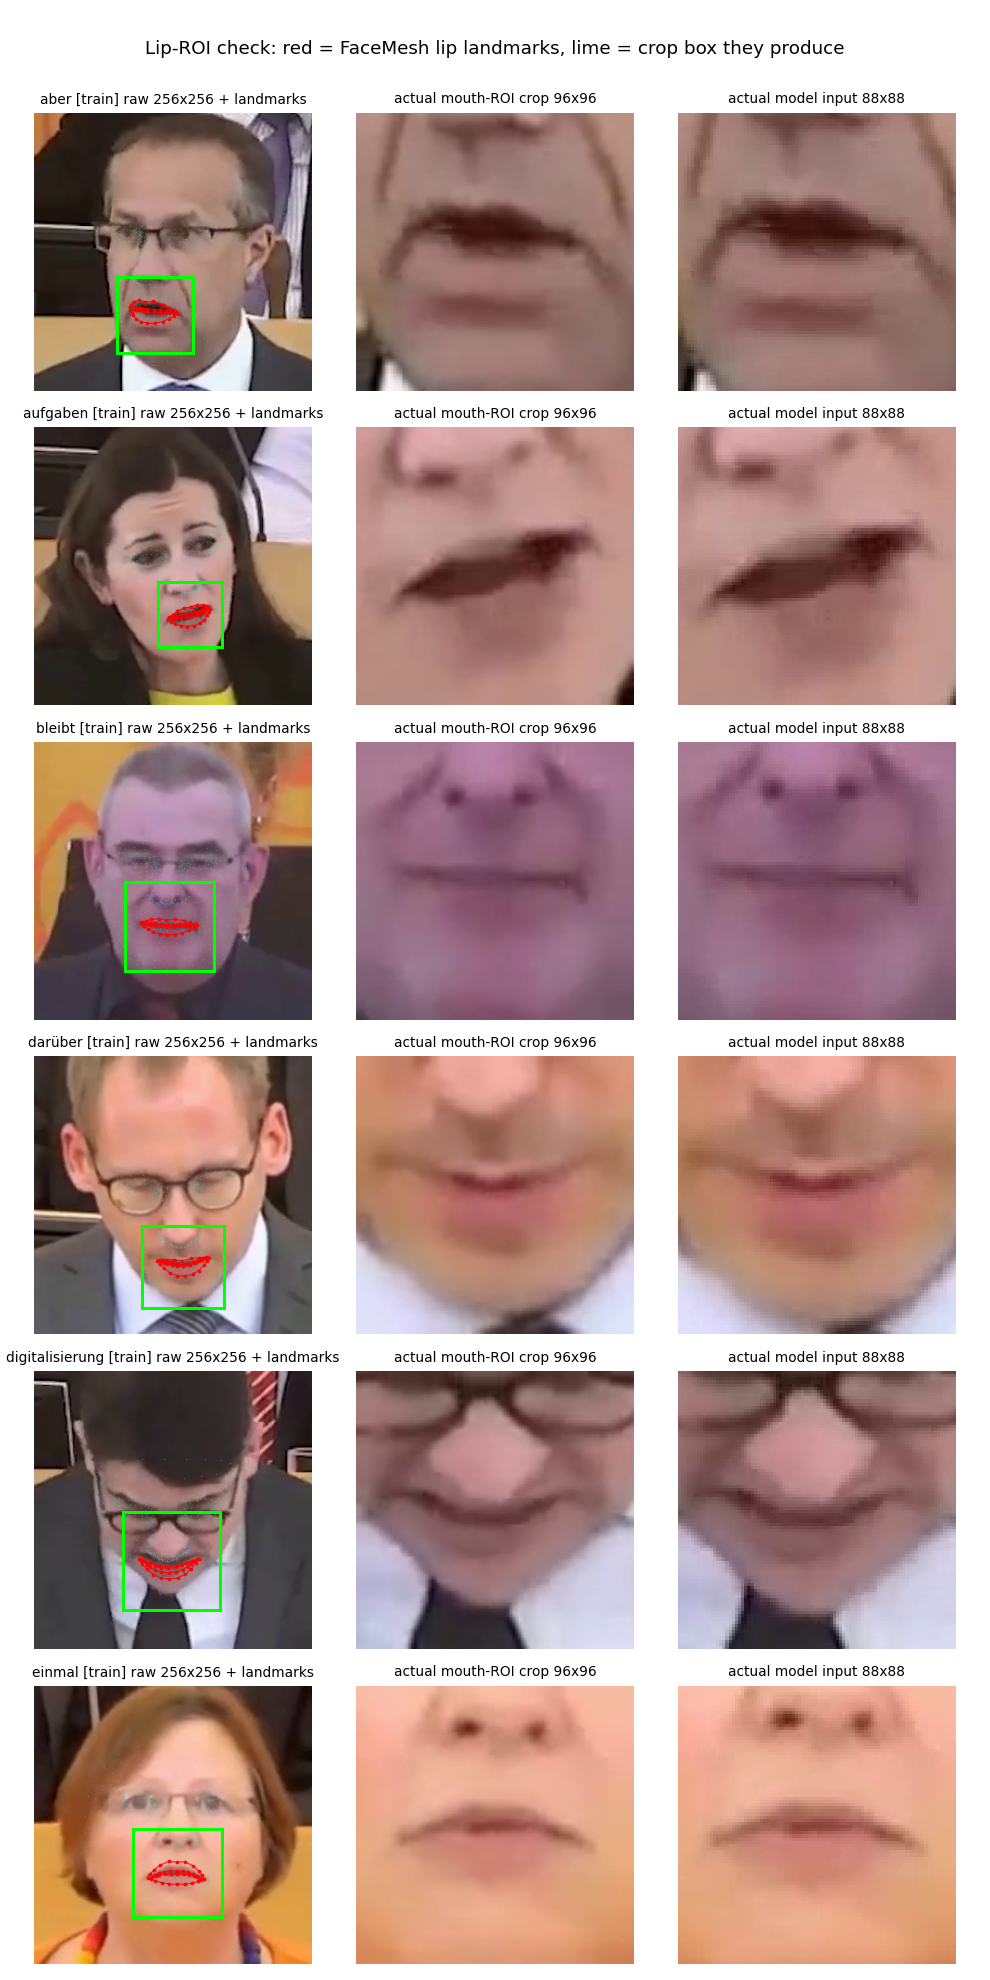
\includegraphics[height=0.5\textheight]{roi_overview.png}
\caption{Mouth-ROI cropping pipeline on six training clips. Left: raw $256\times256$ frame with FaceMesh lip landmarks (red) and the resulting crop box (lime). Centre: the resulting $96\times96$ mouth-ROI crop. Right: the $88\times88$ crop actually consumed by the model after the training-time random crop (centre crop at evaluation).}
\label{fig:roi}
\end{figure}
\paragraph{Baseline-matched pipeline.}
To separate preprocessing from architecture, the input recipe of \citet{ameer2024} is also reproduced on the uncropped frames: no face detection or mouth-ROI crop, each frame resized directly to $128\times128$ with no spatial crop, $16$ frames sampled per clip, per-clip min--max normalisation to $[0,1]$, and random horizontal flipping as the only augmentation. Holding the model and optimiser fixed while switching only between these two pipelines isolates the contribution of the mouth-ROI preprocessing from that of the architecture.
\subsection{Data augmentation}
\label{sec:aug}
\noindent Lip reading depends on the temporal evolution of mouth shape, so the augmentation is built around one invariant: every stochastic transform parameter is drawn once per clip and applied identically to all $T$ frames. A spatial jitter, colour shift or occlusion varying from frame to frame would inject apparent motion unrelated to articulation. All augmentation is active during training only; at validation and test the transform reduces to a deterministic resize, centre crop and normalisation.
\noindent\emph{Geometric.} A single affine warp per clip, with rotation drawn uniformly from $[-10^\circ,10^\circ]$, isotropic scale from $[0.9,1.1]$, and translation up to $6\%$ of the frame along each axis, followed by a random $88\times88$ crop (centre crop at evaluation) and a horizontal flip with probability $0.5$. The affine is applied before the crop so that the crop discards most of the border region the warp introduces.
\noindent\emph{Photometric.} Per-clip brightness and contrast jitter, each a multiplicative factor in $[0.8,1.2]$, and random conversion of the whole clip to grayscale with probability $0.2$. Grayscaling removes a skin-tone and lighting shortcut: because lip reading depends on shape rather than colour, removing the colour channel on a fifth of the clips discourages memorisation of speaker- and studio-specific appearance.
\noindent\emph{Temporal.} Two mechanisms perturb the time axis while holding the frame count fixed at $25$. A speed perturbation resamples the $25$ frames from a randomly warped and offset sub-window of the clip, corresponding to an effective speaking-rate factor in $[0.8,1.2]$, which augments articulation speed and adds a temporal crop. Temporal masking then zeros between one and two contiguous spans of up to $4$ frames each, encouraging the temporal back-end to integrate over the whole utterance rather than rely on a few decisive frames.
\noindent\emph{Occlusion.} With probability $0.25$, random erasing is applied: a single rectangle covering $2$ to $20\%$ of the frame area at aspect ratio in $[0.3,3.3]$ is filled with a flat value. The same rectangle is erased in every frame, consistent with the clip-invariance principle above, simulating partial static occlusion of the mouth.
\subsection{Training setup}
\label{sec:train}
\noindent All models are optimised with AdamW (weight decay $0.05$) under a differential learning rate: the ImageNet-pretrained ResNet-18 backbone is fine-tuned at $\eta_\text{bb}=10^{-4}$, while all freshly initialised parameters (the 3D stem, the temporal module, the positional embedding, the pooling head and the classifier) are trained at $\eta_\text{head}=10^{-3}$. The schedule is a $3$-epoch linear warm-up from $0.1\,\eta$ to $\eta$ followed by cosine annealing. Batch size is $32$, with gradient-norm clipping at $1.0$, and bfloat16 automatic mixed precision, falling back to fp16 with loss scaling where bf16 is unavailable. Every configuration in a given comparison uses identical settings, with the component under test as the only variable.
\noindent For the 15-class runs the full regularisation recipe is used: label smoothing ($\varepsilon=0.1$), batch-level Mixup and CutMix, the augmentation stack of Section~\ref{sec:aug}, and an exponential moving average (EMA) of the weights with decay $0.999$. The EMA weights are used for all validation and checkpoint selection, and the EMA snapshot at peak validation top-1 accuracy is reported as the final checkpoint. These runs are budgeted at $80$ epochs with early stopping on validation top-1 accuracy. For the full-vocabulary runs, which serve as transfer feature sources (Section~\ref{sec:transfer}) and whose classifiers are subsequently discarded, a plain recipe without EMA or Mixup is used, trained for $30$ epochs, which is sufficient for the frontend and temporal back-end to converge as a feature extractor and keeps full-vocabulary training tractable on the available hardware. All experiments are run on a single NVIDIA RTX~3060 ($12$\,GB).
\subsection{Evaluation metrics}
\label{sec:metrics}
\noindent Top-$1$ and top-$5$ classification accuracy and macro-averaged $F_1$ are reported. For $N$ clips with predicted logits $\hat{\mathbf{y}}_i$ and ground-truth label $y_i$, top-$k$ accuracy is
\[
\text{Top-}k = \frac{1}{N}\sum_{i=1}^{N}
\mathbf{1}\!\left[\, y_i \in \operatorname{top\text{-}}k\big(\hat{\mathbf{y}}_i\big) \right],
\]
where $\operatorname{top\text{-}}k(\cdot)$ returns the indices of the $k$ largest logits, with $k=\min(5,C)$ for a $C$-class task. Top-$1$ is the primary metric for model selection and all head-to-head comparisons; top-$5$ characterises near-miss behaviour on a visually confusable vocabulary; macro-$F_1$ is reported because it is the secondary metric used by \citet{ameer2024} and because it is insensitive to the mild class-count imbalance introduced by dropping degenerate classes. Every row of every results table is scored with a single shared evaluation script under one protocol, with the same split, class list and batching, applying each row's own preprocessing.
\subsection{Multimodal data and noise protocol}
\label{sec:mm-data}
\noindent The mouth-crop clips used throughout this paper carry no audio, since cropping discards it; audio for the multimodal experiments is instead read from the sibling, uncropped GLips file for the same clip (identical class, split and filename), which does retain its original audio track. All $498$ classes and the same published train/val/test folders are reused (Section~\ref{sec:pre}), so the multimodal numbers are directly comparable to the visual-only GLips-498 row of Table~\ref{tab:main}: $199{,}203$ training, $24{,}900$ validation and $24{,}900$ test clips. Visual tokens (the pre-pooling GNet output, Section~\ref{sec:arch}) are cached once per split, since the visual encoder is frozen for four of the five multimodal configurations, which is what keeps a full fusion-head training run under four minutes per epoch.
\paragraph{Noise robustness.} To measure how each fusion mechanism behaves as the audio degrades, held-out audio is corrupted with additive white noise or corpus-derived babble noise (the mean of five randomly drawn training-split waveforms) at a controlled per-clip signal-to-noise ratio, at $\{15, 10, 5\}\,$dB in addition to the clean condition, before Whisper encoding. Visual input and the fusion head's weights are unchanged; only the waveform fed to the frozen audio encoder is perturbed. This isolates robustness to acoustic corruption from robustness to visual corruption, which is not evaluated here.
\section{Results}
\label{sec:results}
\noindent All numbers in this section are top-1 and top-5 accuracy and macro-$F_1$ on the held-out GLips \emph{test} folder. Every configuration was trained with a single seed, so gaps of a few points between variants are treated as showing no quantifiable difference in accuracy rather than as one configuration beating another. This caveat applies most to the smaller architectural comparisons below and least to the largest effects, such as the $39$-point multimodal-fusion gap or the $29$-point mouth-ROI effect, which dwarf any plausible run-to-run variation. The 15-word test split also holds only $N=750$ clips against $N=24{,}900$ for the full-vocabulary split, so small differences are harder to resolve there.
\subsection{Main comparison}
\begin{table}[!htb]
\centering
\caption{Test-split results on the published GLips split. Parameter counts correspond to the class count of the row. Chance is $0.2\%$ on GLips-498/500 and $6.7\%$ on GLips-15. Both full-vocabulary rows were updated after a preprocessing bug affecting 2 of 500 classes (`hier', `soll') was fixed: each backbone was warm-started from its original 498-class checkpoint and fine-tuned on the now-complete 500-class split, so macro-$F_1$ was not recomputed for either row. The $\pm$ values are $95\%$ bootstrap confidence intervals (10{,}000 resamples of each trained model's test-set predictions), not multi-seed variance; training remains single-seed throughout (Section~\ref{sec:results}).}
\label{tab:main}
\begin{tabular}{@{}llrrrr@{}}
\toprule
Task & Back-end & Params & Top-1 & Top-5 & Macro-$F_1$ \\
\midrule
GLips-500 & MS-TCN & $17.8$M & $28.9 \pm 0.6$ & $48.5 \pm 0.6$ & -- \\
GLips-500 & GNet   & $13.6$M & $\mathbf{34.2 \pm 0.6}$ & $\mathbf{53.9 \pm 0.6}$ & -- \\
\addlinespace
\multirow{2}{*}{GLips-15 (scratch)} & MS-TCN & $17.6$M & $59.2$ & $\mathbf{86.7}$ & $58.1$ \\
                                    & GNet   & $13.4$M & $59.3$ & $85.7$ & $58.2$ \\
\addlinespace
\multirow{2}{*}{GLips-15 (transfer)} & MS-TCN & $17.6$M & $68.5$ & $\mathbf{89.5}$ & $67.7$ \\
                                     & GNet   & $13.4$M & $\mathbf{69.5}$ & $88.9$ & $\mathbf{69.2}$ \\
\addlinespace
GLips-15 (transfer) & Ensemble & $31.0$M & $\mathbf{70.3}$ & $\mathbf{90.0}$ & $\mathbf{69.8}$ \\
\bottomrule
\end{tabular}
\end{table}
\noindent Table~\ref{tab:main} gives the main comparison, from which three observations follow.
\noindent\emph{On the full vocabulary the Transformer back-end is ahead.} GNet reaches $34.2\%$ top-1 accuracy against MS-TCN's $28.9\%$, a gap of $5.3$ points over $24{,}900$ test clips, and gets there with $4.2$M fewer parameters (macro-$F_1$ was not recomputed for either row on the updated 500-class split, so no macro-$F_1$ comparison is drawn here). This is the largest architectural difference in this study. Both figures are the first reported for the full GLips vocabulary; against a chance rate of $0.2\%$, $34.2\%$ top-1 and $53.9\%$ top-5 accuracy show the task is learnable but far from saturated.
\noindent\emph{On the 15-word task the two back-ends show no quantifiable difference in accuracy.} From scratch they differ by $0.1$ points, and under transfer by $1.0$ points; the top-5 column favours MS-TCN in both rows. No Transformer accuracy advantage is therefore claimed at this vocabulary size. GNet does, however, reach the same accuracy with a $2.9\times$ smaller temporal module.
\noindent\emph{In-domain transfer contributes more than the back-end choice.} Warm-starting from the full-vocabulary model adds $10.2$ points for GNet ($59.3$ to $69.5$) and $9.3$ points for MS-TCN ($59.2$ to $68.5$), an effect an order of magnitude larger than any architectural difference at this scale. A softmax-average ensemble of the two transfer models adds a further $0.8$ points, reaching $70.3\%$; this is reported for completeness, noting that it doubles inference cost for a marginal gain.
\begin{figure*}[!htb]
\centering

\includegraphics[width=\textwidth]{glips500_metrics.png}
\caption{GLips-498: validation accuracy (left, with top-5 as dashed lines) and training accuracy (right) against epoch for the two back-ends. GNet is labelled ``GLipsNet (Transformer)'' in the legend. GNet's peak validation top-1 ($33.4\%$ at epoch~29) exceeds MS-TCN's ($30.8\%$ at epoch~30) throughout most of training, and the top-5 curves separate similarly. This figure shows validation-split curves from the original 498-class training run and was not regenerated after the 500-class fix; the GNet row of Table~\ref{tab:main} reports the updated 500-class model's held-out \emph{test}-split accuracy (val $33.9\%$ at epoch~15 for that run), which is the headline number.}
\label{fig:curves500}
\end{figure*}
\begin{figure*}[!htb]
\centering

\includegraphics[width=\textwidth]{glips15_metrics.png}
\caption{GLips-15, trained from scratch: validation accuracy (left, with top-5 as dashed lines) and training accuracy (right) against epoch. The two back-ends track each other closely throughout, consistent with the test-split result that they are statistically indistinguishable at this vocabulary size; MS-TCN peaks marginally higher ($60.9\%$ at epoch~71 against GNet's $59.5\%$ at epoch~50).}
\label{fig:curves15}
\end{figure*}
\begin{figure*}[!htb]
\centering

\includegraphics[width=\textwidth]{transfer_metrics.png}
\caption{GLips-498 to GLips-15 transfer: validation accuracy (left, with top-5 as dashed lines) and training accuracy (right) against epoch. Both back-ends start above $12\%$ validation accuracy at epoch~1 and peak within $12$ epochs, against roughly $50$--$70$ for the same architectures trained from scratch (Figure~\ref{fig:curves15}), reproducing within GLips the convergence-speed benefit \citet{schwiebert2022glips} report for LRW to GLips transfer. GNet peaks slightly higher on validation top-1 ($72.1\%$ at epoch~12 against MS-TCN's $70.5\%$ at epoch~10).}
\label{fig:curvestransfer}
\end{figure*}
\noindent Figures~\ref{fig:curves500}--\ref{fig:curvestransfer} show the validation and training curves underlying these results. Two features are visible beyond the final accuracies. The back-end curves overlap for most of training on GLips-15 (Figure~\ref{fig:curves15}) and separate steadily on GLips-498 (Figure~\ref{fig:curves500}), consistent with the comparison above. The transfer runs (Figure~\ref{fig:curvestransfer}) also converge considerably faster than the from-scratch runs, peaking within $12$ epochs rather than roughly $50$--$70$, so in-domain pretraining reduces training cost on the target task in addition to improving final accuracy.
\subsection{Comparison with published results}
\begin{table}[!htb]
\centering
\caption{GLips 15-word benchmark against published results. All rows use the corpus's published split. \citet{ameer2024} use the same word set; \citet{schwiebert2022glips} do not publish their draw, so that comparison is approximate.}
\label{tab:sota}
\begin{tabular}{@{}llrr@{}}
\toprule
Method & Pretraining & Top-1 & Macro-$F_1$ \\
\midrule
\citet{schwiebert2022glips}   & none (from scratch)      & $50.9$ & -- \\
\citet{ameer2024} (NASNetMobile + CNN) & ImageNet        & $48.4$ & $48.5$ \\
\citet{schwiebert2022glips}   & LRW (cross-lingual)      & $54.8$ & -- \\
\midrule
GNet                          & ImageNet                 & $59.3$ & $58.2$ \\
GNet                          & ImageNet + GLips-498     & $69.5$ & $69.2$ \\
GNet + MS-TCN ensemble        & ImageNet + GLips-498     & $\mathbf{70.3}$ & $\mathbf{69.8}$ \\
\bottomrule
\end{tabular}
\end{table}
\noindent Table~\ref{tab:sota} places these results against the published literature. The closest comparison is the from-scratch row: with only ImageNet initialisation, as in \citet{ameer2024}, GNet reaches $59.3\%$ against their $48.4\%$, an improvement of $10.9$ points on the same corpus, the same $15$ word classes and the same published split, with a $9.7$-point macro-$F_1$ margin. Adding in-domain GLips-498 pretraining, which uses only GLips training data but more of it than the 15-class training set alone, raises this to $69.5\%$, exceeding the $54.8\%$ that \citet{schwiebert2022glips} obtain by transferring from the larger English LRW corpus.
\noindent Two qualifications apply. First, \citet{schwiebert2022glips} do not report which fifteen words they used, and word-subset difficulty varies considerably, since the first fifteen words alphabetically cap out near $28\%$ in separate runs here, so the comparison against their figures is approximate in a way that the comparison against \citet{ameer2024} is not. Second, in-domain and cross-lingual transfer are not equivalent settings: the source and target here share recording conditions, speakers and language, whereas LRW to GLips transfer must additionally bridge a cross-lingual and cross-corpus gap. The $69.5\%$ figure is therefore best read as establishing a new baseline for in-domain transfer on this benchmark, evidence that in-domain pretraining is a viable alternative for low-resource VSR, rather than as a like-for-like defeat of cross-lingual transfer.
\subsection{Ablations}
\begin{table}[!htb]
\centering
\caption{GNet ablations on GLips-15, test split. Each row is the same architecture and training recipe with a single component changed. $\Delta$ is top-1 accuracy relative to the full model.}
\label{tab:ablation}
\begin{tabular}{@{}lrrrr@{}}
\toprule
Configuration & Top-1 & Top-5 & Macro-$F_1$ & $\Delta$ \\
\midrule
GNet (full)              & $59.3$ & $85.7$ & $58.2$ & -- \\
$-$ attentive pool (mean pool) & $60.5$ & $85.3$ & $60.1$ & $+1.2$ \\
$-$ multi-scale conv stem      & $56.9$ & $83.7$ & $55.9$ & $-2.4$ \\
$-$ mouth-ROI crop             & $30.1$ & $68.1$ & $29.4$ & $\mathbf{-29.2}$ \\
\bottomrule
\end{tabular}
\end{table}
\begin{figure}[!htb]
\centering
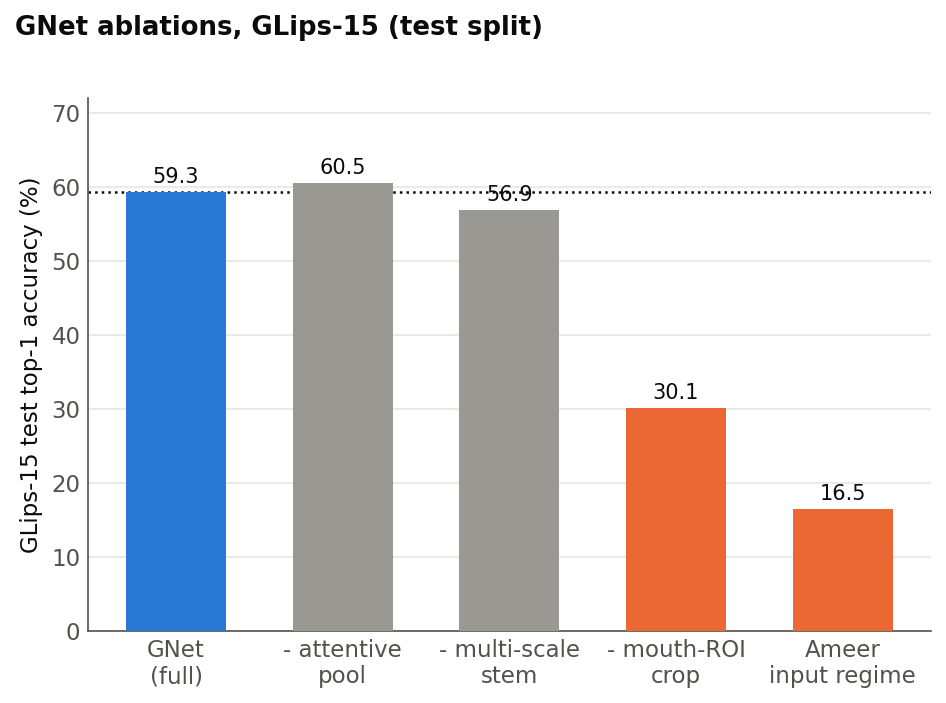
\includegraphics[width=\columnwidth]{fig_ablation.png}
\caption{Test top-1 accuracy for each ablated configuration on GLips-15. The dotted line marks the full model. The two input-pipeline rows, removal of the mouth-ROI crop and the uncropped-input capacity test of Section~\ref{sec:ameer}, account for far larger changes than either architectural component.}
\label{fig:ablation}
\end{figure}
\noindent\emph{Mouth-ROI preprocessing is the dominant factor.} Training the identical model on uncropped full-face frames reduces top-1 accuracy from $59.3\%$ to $30.1\%$, a loss of $29.2$ points, and the only effect in this study larger than a few points. It is roughly $5.5\times$ the size of the largest back-end difference measured here. This indicates that landmark-tracked mouth cropping contributes more on GLips than any temporal-architecture decision evaluated here, and that a corpus of $500$ clips per class does not provide enough data for the model to learn to attend to the mouth region without an explicit cropping stage.
\noindent\emph{The convolutional stem contributes modestly.} Removing it and feeding per-frame features directly into the Transformer costs $2.4$ points. The direction is consistent with the multi-scale receptive-field argument of \citet{martinez2020lipreading} and the stem is retained on that basis, but on this split there is no quantifiable difference in accuracy between the two configurations.
\noindent\emph{Attentive pooling does not outperform mean pooling.} A plain mean-pooling variant scores $1.2$ points higher in top-1 accuracy and $1.9$ points higher in macro-$F_1$. There is no quantifiable difference in accuracy between the two, so they are best treated as equivalent, but the design rationale in Section~\ref{sec:arch}, that attentive pooling should up-weight the articulated frames in an otherwise silent clip, is not supported. One possible explanation is that the augmentation stack already enforces temporal integration, since random temporal masking zeroes short spans specifically to prevent the model from relying on a few decisive frames.
\subsection{Per-class behaviour}
\begin{figure}[!htb]
\centering
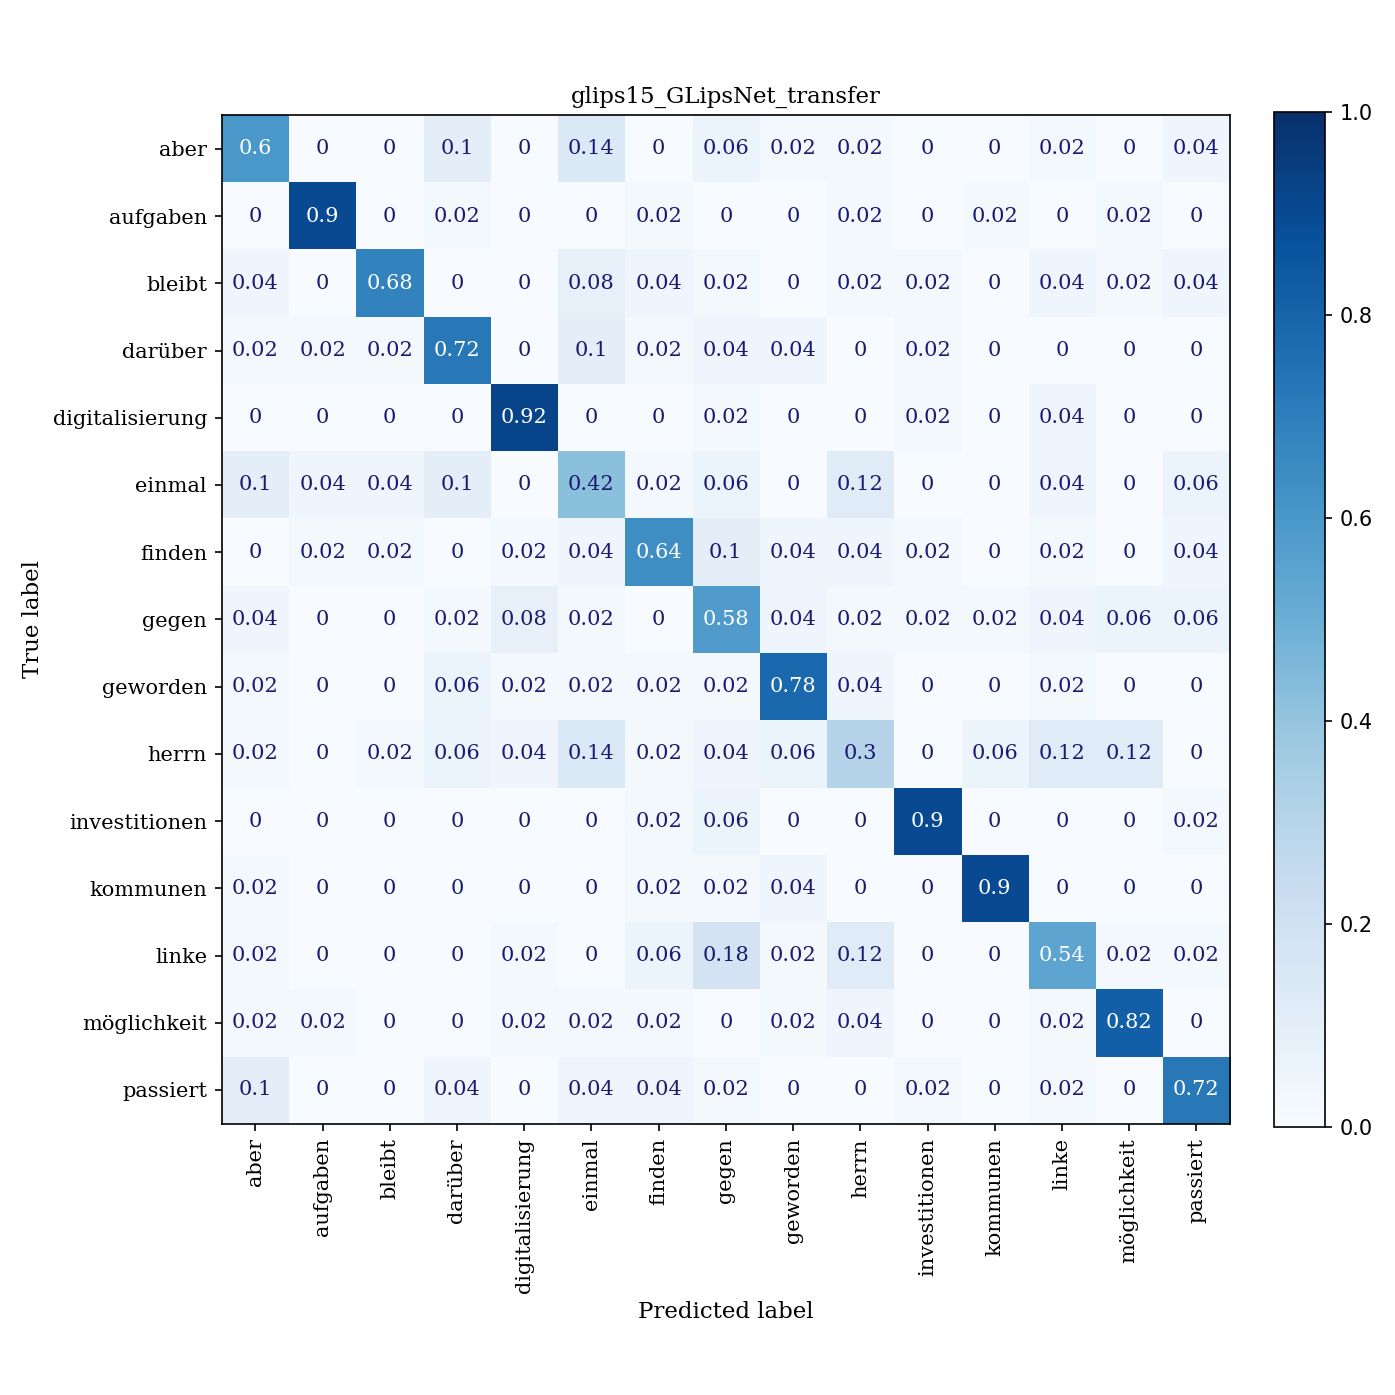
\includegraphics[width=\textwidth]{confusion_matrix.png}
\caption{Row-normalised confusion matrix for GNet with in-domain transfer on the GLips-15 test split. Cells give the rate per true label, so the diagonal is per-class recall. Recall is highest for long, morphologically distinctive words and lowest for short function words, which also account for the largest off-diagonal masses.}
\label{fig:confusion}
\end{figure}
\noindent Figure~\ref{fig:confusion} gives the row-normalised confusion matrix for the best single model. Per-class recall varies widely, from $92\%$ for \emph{digitalisierung} and $90\%$ for \emph{aufgaben}, \emph{investitionen} and \emph{kommunen}, down to $30\%$ for \emph{herrn} and $42\%$ for \emph{einmal}. Recall correlates strongly with orthographic word length (Pearson $r = 0.74$): classes of at least nine characters average $88.0\%$ recall, while those of six characters or fewer average $53.7\%$. \emph{Digitalisierung} is the clearest case: at five syllables it is both the longest word in the set and visually distinctive across its full duration, leaving little room for confusion with any of the shorter words, and it is essentially never confused with anything else in the row. The largest individual confusions are \emph{linke} predicted as \emph{gegen} ($18\%$), and \emph{herrn} and \emph{aber} both predicted as \emph{einmal} ($14\%$ each). \emph{Linke} and \emph{herrn} are also confused with each other in both directions ($12\%$ each way), which is consistent with the two words differing mainly in a tongue articulation (the medial \emph{-nk-} against the rhotic \emph{-rr-}) that produces almost no visible lip movement, leaving the visual signal alone insufficient to separate them reliably. This is consistent with the visual-phonetic structure of the task rather than with a defect of the model: short words span fewer frames and offer fewer distinguishing visemes, and several of the low-recall classes are near-homophenes that are not separable from the lip channel alone. It also indicates that aggregate accuracy on a 15-word subset depends substantially on the length distribution of the words drawn, which is a further reason that comparisons across different word draws, such as the one against \citet{schwiebert2022glips}, should be treated as approximate.
\subsection{GNet capacity versus uncropped inputs}
\label{sec:ameer}
\noindent To test how much of GNet's accuracy depends on the mouth-ROI pipeline rather than on the architecture itself, both back-ends are also trained on uncropped, lower-resolution input: $128\times128$ frames with no face detection or crop, $16$ frames per clip, min--max normalisation, and horizontal flipping as the only augmentation (following the input conventions \citet{ameer2024} use for GLips, minus their choice of a lighter 2D feature-extraction backbone). Under this regime GNet reaches $16.5\%$ top-1 accuracy and MS-TCN $20.9\%$, a severe drop from the $59.3\%$ and $59.2\%$ reached with the full mouth-ROI pipeline (Table~\ref{tab:main}).
\noindent This drop reflects a capacity mismatch rather than a general property of uncropped input. GNet is a $13.4$M-parameter network with a 3D convolutional stem, trained end-to-end with the ResNet backbone fine-tuned; without the mouth-ROI crop and without clip-level augmentation beyond flipping, it overfits severely, reaching $75\%$ training accuracy against $17\%$ on validation, on only $6{,}000$ training clips of uncropped faces. This is the expected failure mode for an end-to-end model of this capacity at this data scale, not evidence that an uncropped, detection-free input regime is inherently harder in general; a lighter, feature-extraction-based pipeline sized to the available data, such as the one \citet{ameer2024} use, need not show the same failure. The result is consistent with the ablation in Section~\ref{sec:results}: GNet's own accuracy is contingent on the ROI crop and the augmentation stack given its capacity relative to the data available, so this experiment is best read as a capacity stress-test of GNet rather than a head-to-head comparison with a differently sized pipeline.
\subsection{Multimodal fusion}
\label{sec:mm-results}
\noindent All numbers in this subsection are on GLips-498, using the same $498$-class published split as Table~\ref{tab:main}; the visual-only and audio-only rows share the exact frozen features consumed by every fusion head, so all seven rows are directly comparable.
\begin{table}[!htb]
\centering
\caption{Multimodal fusion on GLips-498. Params are total parameters exercised at inference (frozen $+$ trainable); the Whisper \emph{base} encoder ($19.8$M, frozen) is common to every audio-consuming row except the fully fine-tuned replica, which uses it identically but is not on cached tokens. Val is used for model selection (early stopping); test is the headline split. The fully fine-tuned cross-attention row was updated after a preprocessing bug affecting 2 of 500 classes (`hier', `soll') was fixed: it was warm-started from the original run and fine-tuned on the now-complete 500-class split; every other row is unchanged and still reflects the original frozen-backbone, 498-class run. That row's $\pm$ is a $95\%$ bootstrap confidence interval (10{,}000 resamples of the single trained model's test-set predictions), not multi-seed variance.}
\label{tab:mm}
\begin{tabular}{@{}lrrrrr@{}}
\toprule
System & Params & Val top-1 & Test top-1 & Test top-5 \\
\midrule
Visual-only (GNet, frozen)     & $13.4$M & $33.3$ & $33.6$ & -- \\
Audio-only (Whisper probe, frozen) & $20.8$M & $61.4$ & $61.0$ & $77.1$ \\
Late fusion                    & $33.6$M & $60.6$ & $60.9$ & $75.5$ \\
Concat fusion                  & $34.2$M & $61.1$ & $61.1$ & $75.7$ \\
Cross-attention (frozen)       & $33.7$M & $71.4$ & $71.9$ & $79.8$ \\
Joint Transformer (frozen)     & $35.9$M & $\mathbf{72.9}$ & $\mathbf{73.0}$ & $\mathbf{80.0}$ \\
\addlinespace
Cross-attention (fine-tuned, end-to-end) & $35.3$M & $72.0$ & $72.0 \pm 0.6$ & $79.7 \pm 0.5$ \\
\bottomrule
\end{tabular}
\end{table}
\noindent\emph{Audio-visual fusion exceeds either unimodal baseline by a wide margin.} The frozen joint Transformer reaches $73.0\%$ top-1 on the test split, against $33.6\%$ visual-only and $61.0\%$ for the audio-only probe on the identical frozen Whisper features ($+39.4$ and $+12.0$ points over $24{,}900$ clips respectively). This is the first published audio-visual figure for GLips at any vocabulary size, and the gap over visual-only exceeds the $29.2$-point mouth-ROI preprocessing effect of Table~\ref{tab:ablation}, the largest effect otherwise measured in this paper.
\noindent\emph{Naive fusion does not use the visual modality at clean audio.} Late and concat fusion score $60.9\%$ and $61.1\%$, indistinguishable in practice from the $61.0\%$ audio-only probe and from each other. Averaging or concatenating pooled features gives the classifier no mechanism to weight vision when audio already carries the answer, so at clean audio these two heads behave as audio-only models that happen to also compute a visual feature. The two attention-based heads do not share this failure: cross-attention reaches $71.9\%$ and the joint Transformer $73.0\%$, $11$--$12$ points above naive fusion, indicating that letting the model attend selectively over the modalities, rather than pooling them, is what is required to extract a fused signal that exceeds either modality alone.
\noindent\emph{The frozen joint Transformer, frozen cross-attention, and the fully fine-tuned cross-attention replica reach closely matched accuracy.} Top-1 accuracy is $73.0\%$, $71.9\%$, and $72.0\%$ respectively, a spread of $1.1$ points across all three. At this margin, drawn from a single trained instance of each system, there is no quantifiable difference in accuracy between them. The joint Transformer is reported as the headline multimodal figure since it has the numerically highest value and uses the same modality-symmetric joint self-attention design as AV-HuBERT, not because a meaningful architectural advantage over cross-attention is established here.
\noindent\emph{A frozen backbone matches full fine-tuning on fused accuracy, but not on the visual-only fallback.} The fully fine-tuned end-to-end replica of the cross-attention architecture ($35.3$M parameters, of which $15.5$M trainable, against $33.7$M total and $0.5$M trainable for its frozen-backbone counterpart) reaches $72.0\%$ test top-1 (updated on the corrected 500-class split, see Table~\ref{tab:mm}), a $0.1$-point gap from frozen cross-attention that shows no quantifiable difference in accuracy between the two. Fine-tuning the backbone therefore does not measurably improve fused accuracy here. It does have a cost: because the fully fine-tuned model's visual pathway was never trained as a standalone classifier, its visual-only fallback (audio dropped at inference) reaches only $26.5\%$, a $7$-point loss relative to the $33.5\%$ floor every frozen-backbone head retains exactly, since freezing the backbone leaves the original visual-only checkpoint's behaviour unmodified. Where a usable visual-only fallback is required, a frozen backbone with a small fusion head is the better-supported choice on these results.
\subsection{Noise robustness}
\label{sec:mm-noise}
\begin{figure*}[!htb]
\centering
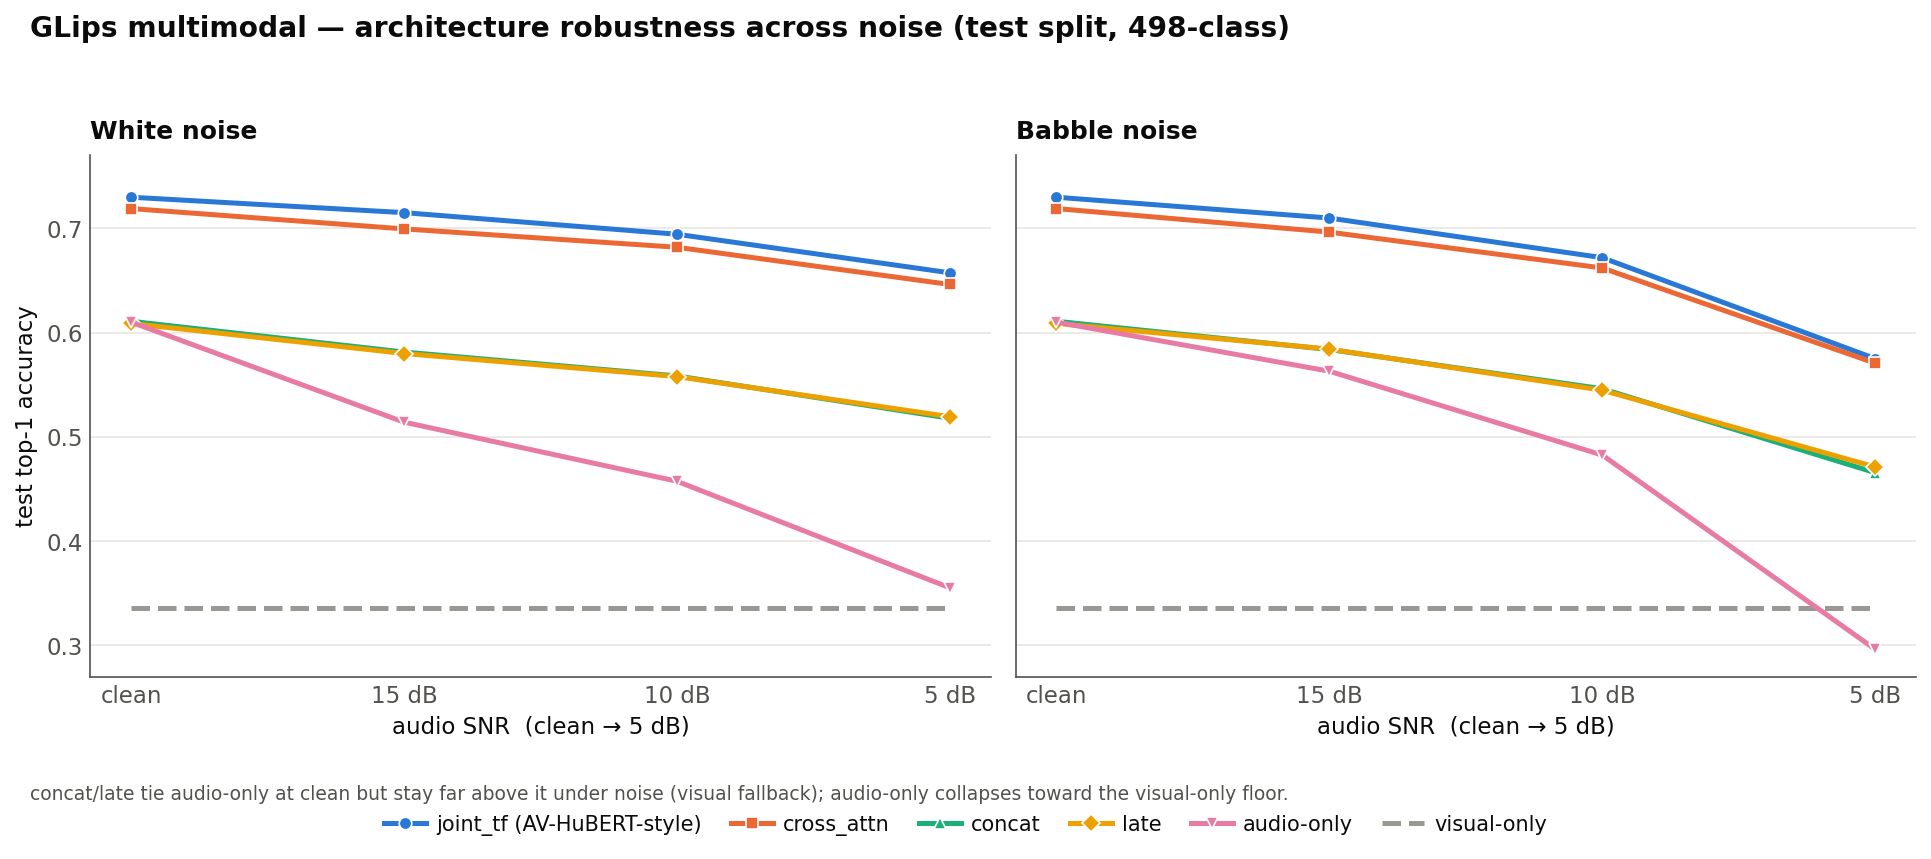
\includegraphics[width=\textwidth]{mm_noise_robustness.png}
\caption{Test-split top-1 accuracy under additive white noise (left) and babble noise (right) at four SNR levels, GLips-498. Attention-based fusion (\texttt{joint\_tf}, \texttt{cross\_attn}) stays well clear of naive fusion (\texttt{concat}, \texttt{late}) at every level; audio-only falls below the flat visual-only floor at the harshest condition tested.}
\label{fig:mm-noise}
\end{figure*}
\noindent Figure~\ref{fig:mm-noise} sweeps the noise protocol of Section~\ref{sec:mm-data} across every fusion head. Three observations follow.
\noindent\emph{Attention-based fusion degrades gracefully and stays ahead of naive fusion throughout.} The gap between the joint Transformer and concat fusion is $11.9$ points at clean audio and remains in the $11$--$14$-point range at every tested SNR ($13.6$ points at $10\,$dB white noise, $10.9$ points at $5\,$dB babble), so attention fusion's advantage is not a clean-audio artefact of the comparison in Section~\ref{sec:mm-results}; it persists under acoustic corruption of the kind that would occur with a distant or interfering speaker.
\noindent\emph{Naive fusion still benefits from its visual fallback under noise, unlike audio-only.} Although concat and late fusion tie the audio-only probe at clean audio, they diverge from it as SNR drops, since their visual pathway is untouched by the noise: at $5\,$dB babble concat reaches $46.6\%$ against audio-only's $29.6\%$, a $17$-point gap that did not exist at clean audio. Naive fusion's failure at clean audio (above) is therefore specifically a failure to use vision when it is not yet needed, not a general inability to use it at all.
\noindent\emph{Audio-only falls below the visual-only floor under the harshest condition.} At $5\,$dB babble noise the audio-only probe scores $29.6\%$, below the $33.6\%$ visual-only floor; at $5\,$dB white noise it scores $35.5\%$, still just above it. Every fusion head, including the two naive ones, remains above both unimodal baselines at every tested condition, so the visual modality's noise-invariance continues to contribute even where naive fusion under-uses it at clean audio.
\section{Discussion and Limitations}
\noindent\emph{The improvement is data-driven rather than architectural.} GNet's $10.9$-point margin over \citet{ameer2024} is a benchmark improvement on a shared split and word set, but the ablations trace it mainly to preprocessing and augmentation, not the temporal back-end. A $29$-point preprocessing effect that exceeds every architectural difference measured here suggests that architectural gains on small VSR corpora are hard to interpret unless preprocessing is held fixed across the compared systems.
\noindent\emph{The Transformer's benefit is limited in scope.} It shows up only at $498$ classes, consistent with self-attention and long-range temporal context mattering more as the label space grows, while at $15$ classes a multi-scale convolutional back-end already captures what the frontend provides. There is no accuracy case here for the Transformer over MS-TCN at small vocabularies; on parameter efficiency it is preferable at any size, and on both counts for large ones.
\noindent\emph{Statistical power is the main methodological limitation.} The published 15-word test split holds only $750$ clips, so small differences are hard to resolve there; several ablations and both 15-word back-end comparisons fall into this range and are marked accordingly. All results are single-seed, so gaps of a few points are reported throughout as showing no quantifiable difference rather than as settled comparisons.
\noindent\emph{Further limitations.} The published split is not speaker-disjoint, so, like \citet{ameer2024} and \citet{schwiebert2022glips} on the same split, these numbers include speaker overlap between train and test and should be read as within-corpus rather than speaker-independent performance. GLips is parliamentary footage: front-facing, well-lit, adult and broadcast-quality. Mouth-ROI cropping suits that setting and may transfer poorly to unconstrained video where face detection fails, the concern \citet{ameer2024} raise for their detection-free design; Section~\ref{sec:ameer} provides no evidence against it. The full-vocabulary models were trained for $30$ epochs under a plain recipe, since they serve as transfer sources, so the $33.5\%$ figure is an initial baseline rather than a ceiling.
\noindent\emph{Multimodal limitations.} The fusion mechanisms operate on two entirely frozen backbones bridged by a lightweight head trained on cached tokens, a computationally efficient design rather than a deep multimodal representation-learning architecture. Read it as a fusion baseline for German audio-visual speech recognition, not a demonstration that the two modalities are jointly optimised at a representational level. That framing fits the finding that the fully fine-tuned end-to-end replica loses $7$ points of visual-only fallback relative to the frozen-backbone design (Section~\ref{sec:mm-results}): jointly fine-tuning both modalities does not improve on the frozen-backbone approach here, and instead costs the visual pathway its standalone competence. The audio encoder is Whisper \emph{base}, pretrained mostly on English and other high-resource languages and used here frozen and unadapted to German, so the $73.0\%$ headline figure is a lower bound on what a German-adapted or jointly pretrained encoder might reach, not a ceiling. Noise robustness is measured under synthetic white and babble noise layered onto otherwise clean parliamentary audio, a controlled proxy rather than genuinely noisy field recordings, and visual corruption (occlusion, poor lighting, off-axis faces) is not evaluated at all. GLips audio is also comparatively clean and single-speaker to begin with, which may understate how much fusion helps, or hurts, in harsher recording conditions. As with the visual-only results, all multimodal numbers here are single-seed.
\section{Conclusion}
\noindent This paper presented GNet, a visual and audio-visual lip-reading architecture for German word-level classification, addressing three gaps in the GLips literature: no full-vocabulary result, no controlled comparison of temporal back-ends, and no audio-visual system on this corpus. GNet's frozen visual encoder was fused with a frozen Whisper audio encoder \citep{radford2022whisper} through a small joint-attention head, a computationally efficient fusion baseline built on two entirely frozen backbones rather than a jointly optimised multimodal architecture, raising GLips-498 top-1 accuracy from $33.5\%$ visual-only to $73.0\%$ on the held-out test split (a $39.5$-point gain over $24{,}900$ clips) and giving the first published audio-visual figure for GLips at any vocabulary size. Under an identical frozen-backbone protocol, attention-based fusion (gated cross-attention and an AV-HuBERT-style \citep{shi2022avhubert} joint Transformer) separates from naive fusion (late score-summation, feature concatenation), which ties an audio-only probe at clean audio and only draws on vision once noise is introduced; under additive white and babble noise, attention-based fusion stays $11$--$14$ points above naive fusion at every condition tested, while the audio-only probe falls below the visual-only floor at the harshest noise level. Freezing both backbones and training only a small fusion head matches a fully fine-tuned end-to-end replica of the cross-attention architecture to within the test set's resolution, while keeping the exact visual-only fallback that end-to-end fine-tuning loses ($7$ points lower), making the frozen-backbone design the better-supported choice whenever a usable unimodal fallback matters.
\noindent The visual model underlying this fusion also improves on the published results for the GLips 15-word benchmark, reaching $59.3\%$ top-1 from scratch against a previous best of $50.9\%$ from scratch and $48.4\%$ for the most recent published pipeline, on the same corpus and split. In-domain GLips-498 transfer lifts this to $69.5\%$, and to $70.3\%$ with a two-back-end ensemble, a new baseline for in-domain transfer on this benchmark rather than a direct comparison to the previously reported $54.8\%$ under cross-lingual LRW pretraining, a different setting evaluated on an unpublished word draw. The first visual-only results on the full GLips vocabulary are also reported, at $34.2\%$ top-1 and $53.9\%$ top-5 across $500$ classes against a chance rate of $0.2\%$ (a corrected 500-class re-run after fixing a preprocessing bug affecting 2 classes; the $33.6\%$ visual-only floor used in the multimodal comparison above predates the fix and is unaffected). The ablations trace this visual improvement mainly to data and preprocessing rather than architecture, with $29.2$ points from mouth-ROI preprocessing and $10.2$ from in-domain transfer, while the Transformer and MS-TCN back-ends are statistically indistinguishable at this vocabulary size; the Transformer leads only on the full-vocabulary task ($5.3$ points), at $2.9\times$ fewer temporal parameters, so it reads as a parameter-efficiency result rather than a general accuracy advantage. The attentive-pooling head, added on the reasoning that most frames in a clip are non-articulatory, also fails to outperform mean pooling.
\noindent These results point toward a German-adapted or jointly pretrained audio encoder in place of an off-the-shelf, English-centric one, real rather than synthetic acoustic and visual corruption for the robustness comparison, and a speaker-disjoint German benchmark large enough to resolve the differences the published split cannot.
\begin{thebibliography}{9}
\bibitem[Afouras et al.(2018)]{afouras2018deep}
T.~Afouras, J.~S. Chung, A.~Senior, O.~Vinyals, and A.~Zisserman.
\newblock Deep audio-visual speech recognition.
\newblock \emph{IEEE Transactions on Pattern Analysis and Machine Intelligence}, 2018.
\bibitem[Ameer et al.(2024)]{ameer2024}
A.~W.~A. Ameer, P.~Salehpour, and M.~Asadpour.
\newblock Deep transfer learning for lip reading based on NASNetMobile pretrained model in wild dataset.
\newblock \emph{IEEE Access}, 12, 2024.
\bibitem[Lee et al.(2025)]{lee2025td3net}
B.~H. Lee, W.~Shin, and S.~W. Han.
\newblock TD3Net: A temporal densely connected multi-dilated convolutional network for lipreading.
\newblock \emph{Journal of Visual Communication and Image Representation}, 111:104540, 2025.
\bibitem[Lugaresi et al.(2019)]{lugaresi2019mediapipe}
C.~Lugaresi, J.~Tang, H.~Nash, C.~McClanahan, E.~Uboweja, M.~Hays, F.~Zhang, C.-L. Chang, M.~G. Yong, J.~Lee, W.-T. Chang, W.~Hua, M.~Georg, and M.~Grundmann.
\newblock MediaPipe: A framework for building perception pipelines.
\newblock \emph{arXiv:1906.08172}, 2019.
\bibitem[Ma et al.(2021)]{ma2021densely}
P.~Ma, Y.~Wang, J.~Shen, S.~Petridis, and M.~Pantic.
\newblock Lip-reading with densely connected temporal convolutional networks.
\newblock In \emph{IEEE/CVF Winter Conference on Applications of Computer Vision (WACV)}, 2021.
\bibitem[Martinez et al.(2020)]{martinez2020lipreading}
B.~Martinez, P.~Ma, S.~Petridis, and M.~Pantic.
\newblock Lipreading using temporal convolutional networks.
\newblock In \emph{IEEE International Conference on Acoustics, Speech and Signal Processing (ICASSP)}, 2020.
\bibitem[Prajwal et al.(2022)]{prajwal2022subword}
K.~R. Prajwal, T.~Afouras, and A.~Zisserman.
\newblock Sub-word level lip reading with visual attention.
\newblock In \emph{IEEE/CVF Conference on Computer Vision and Pattern Recognition (CVPR)}, 2022.
\bibitem[Radford et al.(2023)]{radford2022whisper}
A.~Radford, J.~W. Kim, T.~Xu, G.~Brockman, C.~McLeavey, and I.~Sutskever.
\newblock Robust speech recognition via large-scale weak supervision.
\newblock In \emph{International Conference on Machine Learning (ICML)}, PMLR 202, pages 28492--28518, 2023.
\bibitem[Schwiebert et al.(2022)]{schwiebert2022glips}
G.~Schwiebert, C.~Weber, L.~Qu, H.~Siqueira, and S.~Wermter.
\newblock A multimodal German dataset for automatic lip reading systems and transfer learning.
\newblock In \emph{Language Resources and Evaluation Conference (LREC)}, 2022.
\bibitem[Shi et al.(2022)]{shi2022avhubert}
B.~Shi, W.-N. Hsu, K.~Lakhotia, and A.~Mohamed.
\newblock Learning audio-visual speech representation by masked multimodal cluster prediction.
\newblock In \emph{International Conference on Learning Representations (ICLR)}, 2022.
\bibitem[Stafylakis and Tzimiropoulos(2017)]{stafylakis2017combining}
T.~Stafylakis and G.~Tzimiropoulos.
\newblock Combining residual networks with LSTMs for lipreading.
\newblock In \emph{Interspeech}, 2017.
\end{thebibliography}
\end{document}